\chapter{Pixelové detektory radiace a vyčítací zařízení}	% + pro pixelové detektory
\label{kap:2}
Jednou z možností jak detekovat ionizující záření, patří mimo jiné, použití pixelových detektorů \cite{Grupen_Shwartz_2008}. Pomocí pixelových detektorů, konkrétněji hybridních pixelových detektorů, jsme schopni detailně změřit ionizující záření \cite{Rossi2006}. V této kapitole bude popsána obecná činnost a princip detekce ionizujícího záření za použití pixelových detektorů. V části \ref{Timepix2}, bude detailně popsán detektor z rodiny pixelových detektorů Timepix \cite{Llopart}, detektor Timepix 2 \cite{tpx2_manual}, který je jednou z hlavních součástí této diplomové práce.

\section{Princip činnosti pixelových detektorů}
\label{kap:2.1}
V této části bude popsán obecný princip činnosti pixelových detektorů, který je společný pro všechny detektory radiace z rodiny Timepix \cite{Llopart}, vyvíjenými pod záštitou CERN Medpipix Collaboration \cite{Medpix}. 
\par Pixelový detektor, přesněji hybridní pixelový detektor se skládá ze dvou oddělitelných částí, ze senzorové vrstvy a vrstvy s vyčítací elektronikou viz. obrázek \ref{fig:Timepix}. Právě toto rozdělení na senzorovou a vyčítací část označuje název hybridní detektor.
\par Senzorová vrstva je tvořena polovodičovým materiálem. Důležitými parametry senzorové vrstvy jsou typ polovodičového materiálu a její tloušťka. Nejčastěji používané materiály jsou $\text{Si}$, $\text{CdTe}$ a $\text{GaAs}$. Na senzorovou vrstvu je připojené vysoké napětí, označované jako \textit{bias}. Toto vysoké napětí zajistí vyprázdnění oblasti v polovodičové struktuře senzorové vrstvy. Pokud částice ionizujícího záření interaguje v senzorové vrstvě, dojde k vytvoření volného náboje. Tento náboj je dále zpracován vyčítacím čipem. Vyčítací čip se nachází pod senzorovou vrstvou, která je připojena k této vrstvě za pomocí technologie nazývající se \textit{bump bond}.
\par Vyčítací vrstva (ASIC) je rozdělena na 256x256 individuálních pixelů. Každý pixel obsahuje potřebnou elektroniku ke zpracovaní náboje, vzniklého v senzorové vrstvě. Detailnější popis zpracování analogového náboje na úrovni jednotlivých pixelů, bude popsán pro konkrétní pixelový detektor Timepix 2 v části \ref{Timepix2}. Po analogovém zpracování signálu následuje digitální zpracování. Následně je zpracovaný signál vyveden na výstupní plošky detektoru. Vyčítací vrstva je pomocí \textit{wire bond} technologie připojena k desce plošných spojů viz obrázek \ref{fig:Timepix}. Signály vedoucí z pixelového detektoru jsou následně zpracovány vyčítacím zařízením. Příklady vyčítacích zařízení budou popsány v následující části \ref{Vycitaci zarizeni}.
 \begin{figure}[h!]
 	\centering
 	\captionsetup{justification=centering}
 	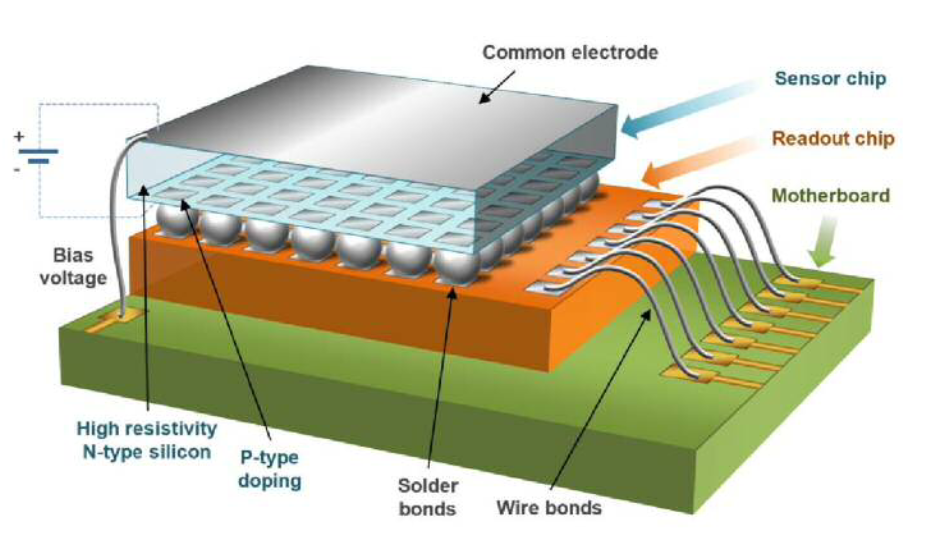
\includegraphics[scale=0.40]{Timepix.png}
 	\caption{Rozložení hybridního pixelového detektoru Timepix \cite{Platkevic}} 
 	\label{fig:Timepix}
 \end{figure}	

\section{Vyčítací zařízení pro pixelové detektory}
\label{Vycitaci zarizeni}
Každý pixelový detektor z rodiny detektorů Timepix \cite{Llopart}, má specifické požadavky pro návrh vyčítacího zařízení. Základními požadavky, kterými jsou napájecí napětí detektoru, komunikační rozhraní detektoru a ovládací rozhraní, musí být splněny, aby bylo možné spolehlivě komunikovat s daným pixelovým detektorem. Vyčítacích zařízení existuje celá řada. V této práci, respektive v následujících částech bude popsán návrh miniaturizovaného vyčítacího rozhraní. Pokusím se tedy především uvést příklady miniaturizovaných vyčítacích zařízení pro pixelové detektory radiace.

\subsection{USB Lite}
Dosud nejmenším vyčítacím zařízením rodiny detektorů Timepix \cite{Llopart}, je zařízení \textit{USB Lite} \cite{usb_lite}, které je zobrazeno na obrázku \ref{fig:usb_lite}. Toto zařízení umožňuje komunikovat s detektorem Medipix 2 \cite{Medpix2}. Rozměry zařízení jsou 60x15 mm. Rychlost vyčítání z pixelového detektoru je 4 fps. Spotřeba zařízení je menší než 2 W \cite{usb_lite}.
 \begin{figure}[h!]
	\centering
	\captionsetup{justification=centering}
	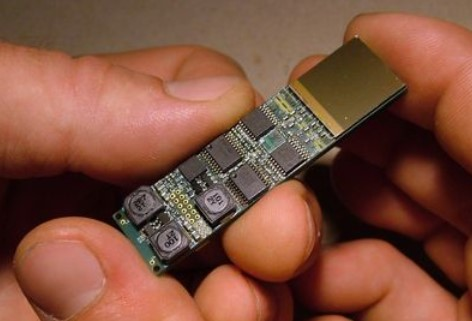
\includegraphics[scale=0.55]{usb_lite.jpg}
	\caption{Vyčítací zařízení \textit{USB lite}} 
	\label{fig:usb_lite}
\end{figure}	

\subsection{MiniPIX SPRINTER}
Vyčítací zařízení MiniPIX SPRINTER je vyvíjeno společností ADVACAM \cite{Advacam}, zařízení je možné vidět na obrázku \ref{fig:sprinter}. Toto zařízení umožňuje komunikovat s pixelovým detektorem radiace Timepix 2 \cite{tpx2_manual}. Rozměry zařízení jsou 80x21x14 mm. Rychlost vyčítání snímků je 99 fps \cite{Advacam}. Uživatelské komunikační rozhraní je USB 2.0 Full Speed s maximální přenosovou rychlostí 12 Mbit/s.
\begin{figure}[h!]
	\centering
	\captionsetup{justification=centering}
	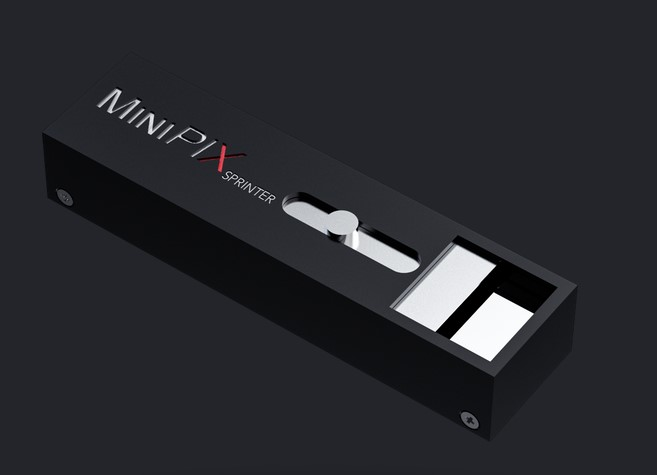
\includegraphics[scale=0.55]{sprinter.jpg}
	\caption{Vyčítací zařízení MiniPIX SPRINTER} 
	\label{fig:sprinter}
\end{figure}	

\subsection{Katherine pro Timepix 2} %katherine zminena protoze modularita
\label{Katherine}
Posledním uvedeným tipem vyčítacího zařízení v této práci je zařízení Katherine pro Timepix 2 \cite{Burian_2020}, které můžete vidět na obrázku \ref{fig:Katherine2}. Toto vyčítací zařízení se od předchozích dvou uvedených liší ve velikosti a maximální vyčítací rychlosti. Katherine pro Timepix 2 se skládá ze dvou částí. Samotným vyčítacím zařízením, na obrázku \ref{fig:Katherine2} vpravo a takzvaným \textit{chipboardem}, na obrázku \ref{fig:Katherine2} vlevo. Část chipboardu obsahuje detektor Timepix 2 a napájecí zdroje potřebné pro provoz detektoru. Dále jsou zde propojeny signály z konektoru od vyčítacího zařízení po samotný detektor Timepix 2. Výhodou tohoto modulárního zapojení je možnost modifikace části obsahující pixelový detektor, bez nutnosti změn na straně vyčítacího zařízení. Tedy existuje možnost k jednomu vyčítacímu zařízení, připojit různé pixelové detektory radiace. Parametry samotného vyčítacího zařízení jsou následující. Rozměry 100x80x28 mm, rychlost vyčítaní až 3.2 Gbps \cite{Burian_2020}.
\begin{figure}[h!]
	\centering
	\captionsetup{justification=centering}
	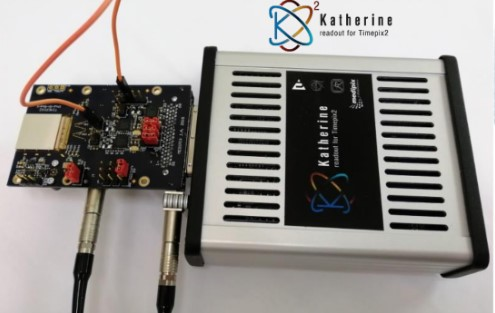
\includegraphics[scale=0.75]{Katherine2.jpg}
	\caption{Vyčítací zařízení Katherine pro Timepix 2 \cite{Burian_2020}} 
	\label{fig:Katherine2}
\end{figure}	

%%%
%%%%%%%%%%%%%%%%%%%%%%%%%%%

\section{Timepix 2}
% v podstatě technická dokumentace Timepix 2, plus konkretni pozadavky pro provoz
\label{Timepix2}
V předchozí části \ref{kap:2.1}, byly popsány obecné vlastnosti pixelových detektoru a základní princip detekce ionizujícího záření. V této kapitole bude detailněji popsán konkrétní detektor, detektor Timepix 2 \cite{tpx2_manual}. Schematické rozložení detektoru Timepix 2 je zobrazeno na obrázku \ref{fig:tpx2_floorplan}. Detektor byl vyvinut pod záštitou CERN Medpipix Collaboration \cite{Medpix}. Timepix 2 patří do rodiny detektorů Timepix. Více o generacích detektorů Timepix lze dohledat například v \cite{Llopart},  \cite{Timepix3} nebo \cite{Timepix4}.  
\begin{figure}[h!]
	\centering
	\captionsetup{justification=centering}
	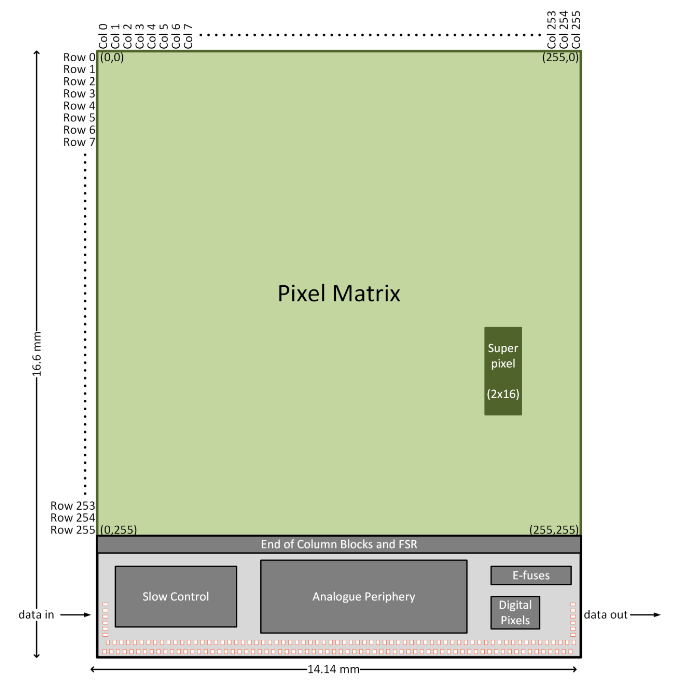
\includegraphics[scale=0.80]{tpx2_floorplan.png}
	\caption{Schematické rozložení detektoru Timepix 2 \cite{tpx2_manual}} 
	\label{fig:tpx2_floorplan}
\end{figure}	

\subsection{Matice pixelů}
Detektor je tvořen maticí 256 x 256 pixelů s roztečí  55 $\mu$$m$. Každý pixel má vlastní analogovou a digitální část, tyto jednotlivé bloky budou popsány v následujících částech \ref{analog} a \ref{Digitálni cast}. Schematické zobrazení jednoho pixelu a jeho analogové a digitální části je možné najít na obrázku \ref{fig:tpx2_cell}.
\subsubsection{Analogová část}	 
\label{analog}
Každý pixel z matice má vlastní analogovou částí, viz. obrázek \ref{fig:tpx2_cell}. Jak bylo zmíněno v kapitole týkající se obecného principu detekce ionizujícího záření \ref{kap:2}, pokud ionizující částice interaguje v senzorové vrstvě dojde k vytvoření volného náboje. Tento náboj je díky připojenému vysokému napětí přitažen k vyčítacím elektrodám. Posbíraný náboj může být charakterizován jako Diracův proudový impuls. Integrací Diracovo proudového impulsu poté dostaneme celkový generovaný náboj Q. 
\par Analogové zpracování signálů na úrovni jednotlivých pixelů probíhá následovně. Diracův proudový impuls vytvořený na senzorové vrstvě je naintegrován do malého vstupního kapacitoru $C_{FB}$ z obrázku \ref{fig:tpx2_cell}. Poté na výstupu CSA je v ideálním případě napěťový skok s amplitudou Q/Cf viz. \ref{fig:tpx2_cell}. Výstupní napěťový pulz je poté porovnán s prahovou úrovní. Nastavením prahové úrovně lze eliminovat úroveň šumu a zbytkový proud, takzvaný \textit{leakage current}, závěrného směru polovodičové struktury, který zde vznikl kvůli připojenému vysokému napětí a současně s tím i nekvalitou připojeného senzoru. Pokud je výstupní signál větší než daná nastavená úroveň, je inkrementován digitální čítač \cite{Llopart}. Každý diskriminátor obsahuje 5-bitový DAC převodník, tento převodník umožňuje nastavit úroveň detekovatelného signálu pro každý pixel individuálně a tím lokálně eliminovat šum způsobený zbytkovým proudem polovodičové struktury a nekvalitou připojeného senzoru.
\par Pokud není povolena funkce adaptivního zesílení signálu, ve zpětné vazbě CSA z obrázku \ref{fig:tpx2_cell} je fixní hodnota kondenzátoru $C_{FB}$. Tedy dochází k rovnoměrnému zesílení vstupního signálu, bez ohledu na velikosti generovaného náboje. 
\par Pokud je povolen režim adaptivního zesílení, zpětná vazba CSA je tvořena kondenzátorem $C_{FB}$ paralelně s kapacitou MOS tranzistoru z obrázku \ref{fig:tpx2_cell}. Zesílení vstupního signálu je poté větší pro vstupní signály s malou amplitudou a nižší pro signály s vysokou amplitudou, více o této metodě lze dohledat například v \cite{MOS}.
\begin{figure}[h!]
	\centering
	\captionsetup{justification=centering}
	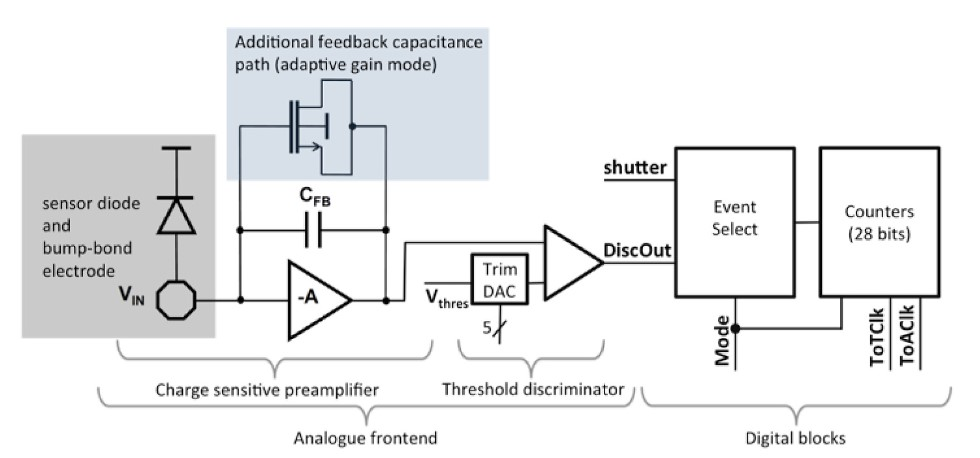
\includegraphics[scale=0.70]{tpx2_cel.jpg}
	\caption{Uspořádání jednoho pixelu \cite{Timepix2}}
	\label{fig:tpx2_cell}
\end{figure}

\subsubsection{Digitální část}
\label{Digitálni cast}
Zobrazení digitální části jednotlivých pixelů, je možné vidět na obrázku \ref{fig:tpx2_cell}. Každý pixel obsahuje digitální čítače o celkové délce 28 bitů. Konkrétně se jedná o čtyři digitální čítače typu LSFR. V případě Timepix 2 každý pixel obsahuje dva 10-bitové (označení: A,B) a dva 4-bitové (označení: C,D) čítače. Například 14-bitový čítač lze jednoduše vytvořit kombinací 10-bitového a 4-bitového čítače. Díky použití lineárně posuvného čítače LSFR, každý n-bitový čítač generuje $2^n$ pseudonáhodných čísel. Odpovídající dekódovaná hodnota pseudonáhodného čísla lze pro příklad čtrnácti bitového čítače získat za použití rovnice \ref{eq:1}. To jaká hodnota bude uložena do konkrétního čítače určují jednotlivé digitální režimy detektoru, které budou popsány následovně.
\begin{equation}
	14bit = (hodnota_{4bit} \cross 2^{10}) + hodnota_{10bit}
	\label{eq:1}
\end{equation}
Jak bylo zmíněno výše. Digitální čítače můžou bát nakonfigurované do různých měřících módů. Pro Timepix 2 jsou to následující módy \ref{fig:modes}. 
\begin{itemize}
	\item \textbf{Time over Threshold} (ToT): Čítač je inkrementován při každém hodinovým pulsu, kdy je signál nad nastavenou prahovou úrovní
	\item \textbf{Time of Arrival} (ToA): Čítač je inkrementován při každém hodinovým pulsu, od okamžiku, kdy signál překročí nastavenou úroveň a inkrementuje se až do konce akvizice.
	\item \textbf{Coutnig mode}: Čítač je inkrementován právě o jedna, pokud došlo k překročení nastavené prahové úrovně detekce.
\label{item:modes}
\end{itemize}
\begin{figure}[h!]
	\centering
	\captionsetup{justification=centering}
	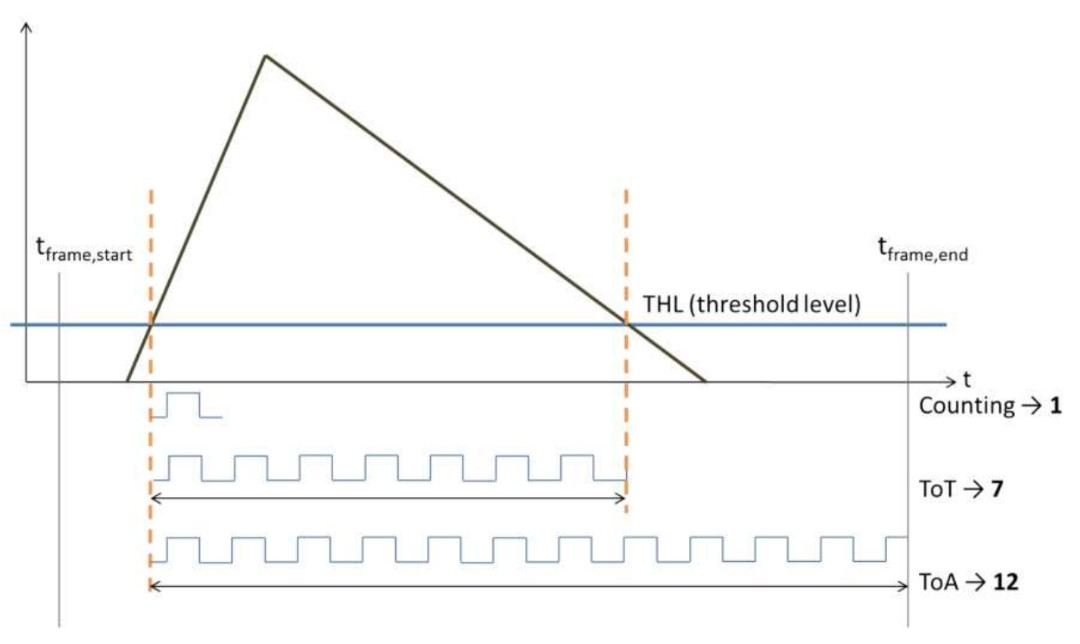
\includegraphics[scale=0.45]{modes.jpg}
	\caption{Digitální módy Timepix 2 \cite{Manek}} 
	\label{fig:modes}
\end{figure}	
\par Celkem lze použít 8 digitálních módu. Každý jednotlivý mód určuje, jaká informace bude v jakém čítači uložena. Například při použití digitálního módu s označením ToT10/ToA18  je do 10 bitového čítače ukládána informace ToT a do 18 bitového čítače je ukládána informace ToA. Více o jednotlivých digitálních módech Timepix 2 lze dohledat v technické dokumentaci \cite{tpx2_manual}.

\par Digitální čítače mimo výše popsaných digitálních módů můžou pracovat buď v simultánním, nebo kontinuálním režimu. Simultánní režim znamená, že naměřená data musí být vždy vyčtena z 28 bitového digitálního čítače, přičemž při vyčítání není možné měřit příchozí ionizující záření. Doba kdy detektor nemůže měřit vlivem samotného vyčítaní dat se nazývá mrtvá doba detektoru. Pro Timepix 2 při použití sériového komunikačního rozhraní s frekvencí hodinového signálu 100 MHz je tato doba přibližně 18.3 ms. Druhým režimem je režim kontinuální. Výhodou kontinuálního režimu je, že zde je kratší mrtvá doba, v závislosti na použitém čítači 6.5 ms až 9.2 ms . Zjednodušený princip činnosti je, že dva digitální čítače jsou nastaveny na stejnou velikost, přičemž do jednoho z čítačů se ukládá informace o měření, dle nastaveného měřícího módu. Tento čítač je zřetězení s druhým čítačem. Druhý čítač slouží pouze pro vyčtení informace o měření. Doba vyčtení tohoto čítače poté definuje výše uvedenou mrtvou dobu.
\par Příkladem použití digitálního módů může být způsob měření energie, kterou interagující částice zanechala v senzoru. Tuto energii můžeme zjistit pokud vybereme digitální mód, při kterém se do některého z čítačů ukládá informace o ToT měření. Následně počet naměřených hodinových pulsů odpovídá času, pro který hodnota analogového napětí měřeného signálu byla nad nastavenou detekovatelnou úrovní. Více o způsobu měření energie, lze dohledat například v \cite{JAKUBEK2011S262}.

\subsection{Technická specifikace} %napáječky, kom. rozhraní, prikazy atd.., VN, hodiny pro měření, I/O piny
\label{Technicka specifikace}
Timepix 2 je rozdělen do 256 x 256 pixelů. Rozteč mezi jednotlivými pixely je 55 $\mu$$m$. Celkově rozměry Timepix 2 jsou 16.6 x 14.14 mm. Vyčítací část detektoru tvoří ASCI čip navržen ve 130 nm CMOS technologii. Samotná výroba ASIC je zajišťována jedním z předních výrobců čipů, firmou TSMC \cite{TSMC} na Taiwanu. Všechny technické informace, nebude-li uvedeno jinak jsou čerpány z manuálu k detektoru Timepix 2 \cite{tpx2_manual}.

\subsubsection{Komunikační rozhraní}
\label{Komunikacni rozhrani}
Timepix 2 umožňuje komunikaci za použití paralelního nebo sériového rozhraní. Při použití paralelního rozhraní je možno využít 32 paralelních datových vodičů. Paralelní rozhraní dosahuje násobně vyšších přenosových rychlostí v závislosti na počtu použitých paralelních vodičů. Tuto závislost je možné vidět na obrázku \ref{fig:rychlosti}. Pro paralelní zpracování dat je zapotřebí na straně vyčítací elektroniky použít velmi rychlé rozhraní, například FPGA.  
\par Sériová komunikace probíhá po diferenciálních datových párech. Konkrétně se jedná o komunikační specifikaci SLVS \cite{SLVS}. Napěťové úrovně této specifikace lze najít na obrázku \ref{fig:SLVS_LVDS}. Jak lze z obrázku \ref{fig:SLVS_LVDS} vidět, specifikace SLVS je analogická ke komunikační specifikaci LVDS \cite{LVDS}. Výhodou specifikace SLVS oproti LVDS jsou především menší napěťové komunikační napěťové úrovně a s tím spojený menší odebíraný výkon. Maximální frekvence komunikačních hodin při použití sériového rozhraní je dle manuálu Timepix 2 \cite{tpx2_manual} 100 Mhz. Z uvedených parametrů týkající se maximální rychlosti komunikace, lze na straně vyčítacího rozhraní navrhnout například použití mikroprocesoru. Hlavní nevýhodou sériové komunikace je limitovaná maximální přenosová, která je násobně nižší než za použití paralelního rozhraní \ref{fig:rychlosti}. Naopak výhodou sériové komunikace jsou především jednoduchost implementace.
\begin{figure}[h!]
	\centering
	\captionsetup{justification=centering}
	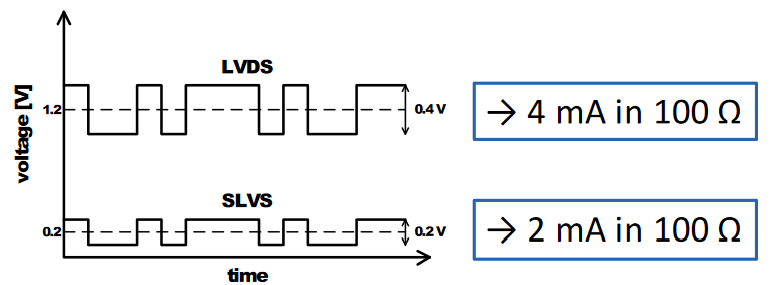
\includegraphics[scale=0.55]{SLVS_LVDS.png}
	\caption{SLVS specifikace \cite{SLVS}} 
	\label{fig:SLVS_LVDS}
\end{figure}	

\subsubsection{Napájení}	
Timepix 2 ke své činnosti potřebuj celkem 3 napájení viz. tabulka \ref{tab:tpx2_napajeni}. Napájení VDD slouží pro napájení digitální části jádra Timepix2 a VDDA slouží k napájení analogové části jádra Timepix 2. Napájení VDDIO slouží k napájení vstupních/výstupních bran detektoru. Posledním uvedeným napájení v tabulce \ref{tab:tpx2_napajeni} je napájení VDD33. Toto napájení je potřeba přepínat, podle potřebné funkcionality detektoru. Pokud chceme z Timepix 2 vyčíst CHIP ID, musíme na pin VDD33 aplikovat napájecí napětí 2.5 V. Při ostatní činnosti detektoru, je požadováno aby napětí označené VDD33 bylo 1.2 V. 
\begin{table}[h!]
	\centering
	\begin{tabular}{ |P{3cm}||P{5cm}||P{3cm}|  }
		\hline
		\multicolumn{3}{|c|}{Napájecí úrovně Timepix 2} \\
		\hline
		Název pinu& Hodnota napájecího napětí [V] & Počet pinů\\ \hline \hline 
		VDDIO & 2.5 & 7\\ \hline		
		VDD & 1.2 & 15\\ \hline 		 
		VDDA & 1.2 & 18\\ \hline
		VDD33 & 2.5 (1.2)& 1\\ \hline
	\end{tabular}
	\caption{Napájecí úrovně Timepix 2}
	\label{tab:tpx2_napajeni}
\end{table}
\par Speciální kategorií napájení je vysoké napětí zajištující vyprázdnění oblasti v senzorové vrstvě, které je připojeno právě na tuto vrstvu. Toto napětí zajistí vyprázdnění oblasti v polovodičové struktuře. Požadavky na parametry vysokého napětí záleží na typu, polaritě a tloušťce senzorové vrstvy. Nejčastěji používaným materiálem senzorové vrstvy je křemík, ovšem záleží na příkladu použití detektoru. Uvedu-li příklad vysokého napětí, které bylo použito pro testování Timepix 2 s křemíkovou senzorovou vrstvou o tloušťce 500 $\mu$m dle \cite{Timepix2_500um} bylo 100 V. Další příklady velikosti vysokého napětí používaných pro různé senzorové vrstvy lze najít v odkazech \cite{Timepix_500um_Pospisil}, \cite{Timepix_500um_Huston}. Důležitou vlastností vysokonapěťových zdrojů je možnost nastavení výstupního vysokého napětí v určitém pracovním rozsahu rozsahu.   

\subsubsection{Spotřeba}	
Celková spotřeba Timepix 2 dle \cite{Timepix2} při zapnutí všech pixelů a frekvenci datových hodin $f_{clock}$ = Mhz je nižší než 900 mW. Přičemž spotřeba jednoho pixelu je 5 $z\mu$A.
\par Timepix 2 disponuje možnostmi, jak celkovou spotřebu detektoru snížit. Ke celkovému snížení spotřeby slouží funkcionalita, která umožňuje zamaskovat pixely, které nebudou dále použity pro ukládání informace z měření. Zamaskovat lze individuální pixely detektoru nebo takzvané super pixely, které jsou označeny jako sdružení 2x16 jednotlivých pixelů. Při zamaskování dojde k téměř kompletnímu vypnutí vybraných pixelů. Z výše uvedené spotřeby pro jeden pixel, se pro vybraný pixel, který má být zamaskovaný, dostáváme na spotřebu okolo jednotek nA na jeden pixel.

\subsubsection{Rychlost komunikace}
V části \ref{Komunikacni rozhrani}, byly popsány možnosti využití paralelního, či sériového rozhraní pro komunikaci s Timepix 2. Doba pro vyčtení celé matice pixelů pro oba typy rozhraní lze vidět na obrázku \ref{fig:rychlosti}. 
\begin{figure}[h!]
	\centering
	\captionsetup{justification=centering}
	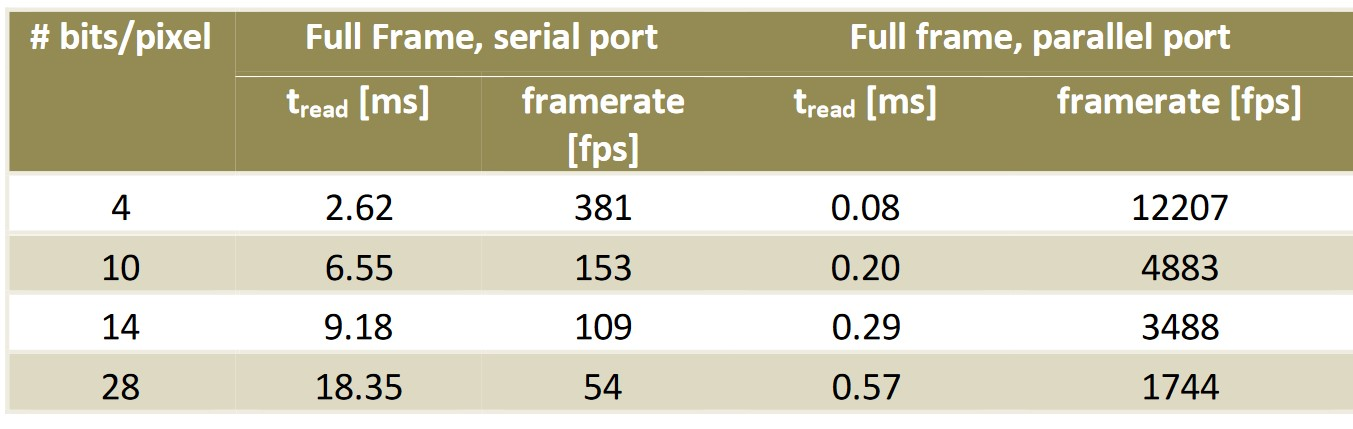
\includegraphics[scale=0.65]{rychlosti.jpg}
	\caption{Vyčítací rychlosti snímků z Timepix2. Frekvence hodin $f_{clock}$ = 100 MHz \cite{Timepix2}} 
	\label{fig:rychlosti}
\end{figure}	

Poslední možností vyčítání dat z Timepix 2 je použití ZCS módu. Tento mód lze použít při vyčítání dat přes sériové rozhraní. Na obrázku \ref{fig:rychlosti}, lze vidět, že tento mód je rychlejší než použití sériového rozhraní při vyčítání celých snímku. Při použití ZCS módu nejprve detektor odešle 256 bitů, které odpovídají jednotlivým sloupcům detektoru. V těchto 256 bitech je uložena informace o tom, zda-li došlo v příslušném sloupci k detekci ionizujícího záření, neboli jestli byl zasažen alespoň jeden pixel v tomto sloupci. Pokud ano, bude sloupec nastaven na logickou hodnotu 1. V opačném případě zůstává hodnota sloupce v logické nule. Po obdržení 256 bitů je přijato tolik dat, kolik sloupců bylo zasaženo. Avšak minimální počet odeslaných sloupců je 16 a to i v případě, pokud by nebyla detekována žádná částice v celé matici. Velikost poslaných dat za použití ZCS módu je tedy vždy závislá na aktivitě ionizujícího záření a s tím i spojená vyčítací rychlost. Pokud by byly aktivovány všechny pixely, bude rychlost ZCS módu nanejvýše stejně rychlá, jako při vyčtení celého snímku. Na obrázku \ref{fig:rychlosti} je pro ZCS mód uvažováno vyčtení 16 sloupců matice.


\subsubsection{Rozhraní pro připojení Timepix 2 k desce plošných spojů}
Připojení Timepix 2 k desce plošných spojů je nejčastěji realizováno pomocí technologie \textit{wire bonding}. Timepix 2 má celkem 152 pinů pro připojení wire bondů. Rozložení pinů je zobrazeno na obrázku \ref{fig:tpx2_floorplan} ve spodní části. Rozteč mezi jednotlivými piny je 108 $\mu$m.

\par Dalším možným způsobem připojení Timepix 2 k desce plošných spojů je technologie zvaná TSV. Pomocí této technologie je možné signály vyvést ze zadní strany Timepix 2 k pájecím ploškám. Vznikne tím tak uspořádání, známe z technologie výroby pouzder BGA elektronických součástek. 
\par Běžnější způsob připojení Timepix 2 k desce plošných spojů je pomocí wire bondů. Použití wire bondů i technologie BGA je možné vidět na obrázku \ref{fig:bga}. Výhodou technologie BGA oproti technologii wire bondů je lepší praktické zacházení s detektorem, díky absenci tenkých wire bondů, které jsou velmi náchylné na mechanické poškození. Další výhodou je poté technologicky méně náročné připojení detektoru k desce plošných spojů. Nevýhodou této technologie je vystavení chipu vysoké teplotě při pájení detektoru na desku plošných spojů.
\begin{figure}[h!]
	\centering
	\captionsetup{justification=centering}
	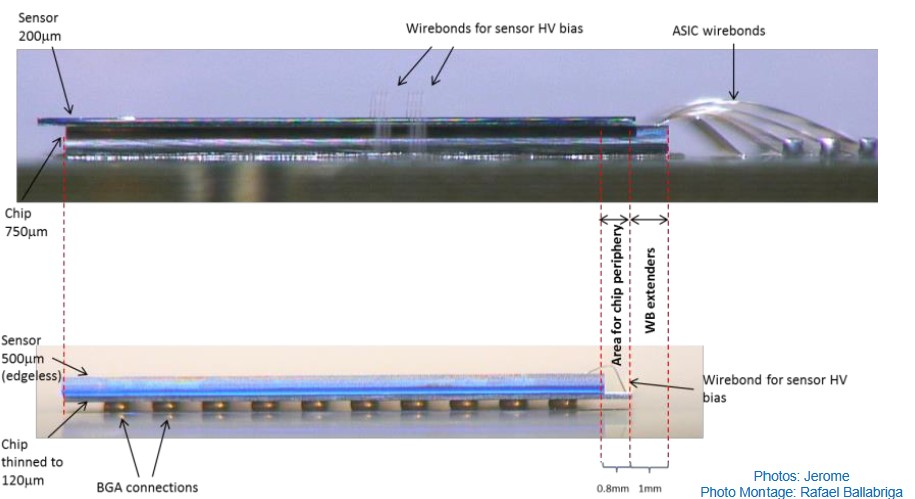
\includegraphics[scale=0.55]{bga.jpg}
	\caption{Připojení detektoru Timepix 2 k desce plošných spojů \cite{TSV}} 
	\label{fig:bga}
\end{figure}	









